\documentclass[11pt,a4paper]{amsart}
\usepackage[utf8]{inputenc}
\usepackage[T1]{fontenc}
\usepackage{lmodern}
\usepackage{amsmath,amssymb,amsthm}
\usepackage{booktabs}
\usepackage{graphicx}
\usepackage{xcolor}
\usepackage[margin=2.6cm]{geometry}
\usepackage[colorlinks=true,linkcolor=blue!50!black,citecolor=blue!50!black,urlcolor=blue!50!black]{hyperref}
\graphicspath{{../figures/}}

\newtheorem{theorem}{Theorem}[section]
\newtheorem{proposition}[theorem]{Proposition}
\newtheorem{lemma}[theorem]{Lemma}
\newtheorem{corollary}[theorem]{Corollary}
\theoremstyle{definition}
\newtheorem{definition}[theorem]{Definition}
\theoremstyle{remark}
\newtheorem{remark}[theorem]{Remark}

\newcommand{\F}{\mathbb{F}}
\newcommand{\Z}{\mathbb{Z}}
\newcommand{\Tr}{\operatorname{Tr}}
\newcommand{\disc}{\operatorname{disc}}
\newcommand{\Res}{\operatorname{Res}}
\newcommand{\AGL}{\mathrm{AGL}}
\newcommand{\GL}{\mathrm{GL}}

\title[{Oppermann intervals in $\F_q[t]$}]{Oppermann intervals in $\F_q[t]$:\\
counterexamples in characteristic~$2$ and a computer-assisted theorem in odd characteristic}
\author{Ruqing Chen}
\address{GUT Geoservice Inc., Montreal, Canada}
\email{ruqing@hotmail.com}
\thanks{Draft, October 2026. Code and data in the accompanying repository (directories \texttt{code/}, \texttt{data/}).}
\date{\today}

\begin{document}

\begin{abstract}
For a monic $f\in\F_q[t]$ of degree $d$ the Legendre interval $\{f^2+s:\deg s\le d\}$ splits into the $q$
\emph{Oppermann sub-intervals} $O_{f,c}=\{f^2+cf+s:\deg s<d\}$, $c\in\F_q$, each of size $q^d$; for $q=2$ these are
the two halves, the analogue of $(n^2,n^2+n)$ and $(n^2+n,(n+1)^2)$. We ask whether every $O_{f,c}$ contains an
irreducible polynomial. In characteristic~$2$ the answer is no, and the failures are explained completely by three
Galois-theoretic obstructions: (A)~for $d=1$ the piece $c=0$ consists of squares; (B)~for $d=2$ we compute the exact
number of irreducibles in every Oppermann sub-interval, $q^2/4$, $0$, $q(q-2)/4$ or $q(q-1)/2$, by letting Frobenius act
on the roots of an additive polynomial through $\AGL_2(\F_2)\cong S_4$; it vanishes exactly when $q=4^j$, $a_1^2+c=0$, or
$q=2$, $a_1^2+c=1$; (C)~for $q=2$, $d=4$ the block $\{t^8+s:\deg s\le3\}$ contains no irreducible, by the
Stickelberger--Swan sign of Frobenius, because $8\mid\deg$ makes the sign depend only on the tail. In odd
characteristic every class of the Hayes group of level $d$ is an Oppermann sub-interval, and an exact computation
with the Hayes explicit formula shows that all of them contain irreducibles for $q=3$, $d\le16$; $q=5$, $d\le10$;
$q=7$, $d\le9$; $q=9$, $d\le8$; $q=11$, $d\le7$; $q=13$, $d\le6$. In characteristic~$2$ the same computation, for
$q\in\{2,4,8,16\}$ up to $q^d\le2^{26}$, finds no empty Oppermann sub-interval beyond (A)--(C). The Weil bound sits
exactly at the square-root barrier for these intervals and cannot prove nonemptiness for any $d\ge2$.
\end{abstract}

\maketitle

\section{Introduction}

Oppermann's conjecture \cite{Oppermann} asserts that for every $n\ge2$ both $(n^2,n^2+n)$ and $(n^2+n,(n+1)^2)$
contain a prime. It implies Legendre's conjecture and lies beyond the Riemann hypothesis, which gives primes only
in intervals $[x,x+C\sqrt x\log x]$. Over $\F_q[t]$, Legendre intervals $I_f=\{f^2+s:\deg s\le d\}$ ($f$ monic of
degree $d$) were studied in \cite{ChenI}. Since $f^2+cf$ and $f^2+ct^d$ differ by a polynomial of degree $<d$, the
interval $I_f$ is the disjoint union of the $q$ sub-intervals
\begin{equation}\label{eq:Ofc}
O_{f,c}=\{f^2+cf+s:\deg s<d\}=\{f^2+ct^d+s:\deg s<d\},\qquad c\in\F_q,
\end{equation}
each of cardinality $q^d=|f|$, the norm of $f$, exactly as $(n^2,n^2+n)$ has length $n$. For $q=2$ there are two
halves. We call $O_{f,c}$ the \emph{Oppermann sub-intervals} and ask:

\begin{quote}
\emph{Does every $O_{f,c}$ contain an irreducible polynomial?}
\end{quote}

\noindent The answer depends on the characteristic.

\begin{theorem}[characteristic $2$]\label{thm:main2}
Let $q=2^k$.
\begin{enumerate}
\item[(A)] For $d=1$ the $q$ sub-intervals $O_{f,0}$ consist of squares.
\item[(B)] For $d=2$ and $f=t^2+a_1t+a_0$, the number of irreducibles in $O_{f,c}$ depends only on $e=a_1^2+c$ and
equals
\[
\begin{array}{c|cc}
 & e=0 & e\ne0\\\hline
k\text{ even} & 0 & q^2/4\\
k\text{ odd} & q(q-1)/2 & q(q-2)/4
\end{array}
\]
The table has two zero entries: $k$ even with $e=0$, and $q(q-2)/4$ at $q=2$ (where $k=1$ is odd). Hence
$O_{f,c}$ is empty if and only if either $k$ is even and $c=a_1^2$, or $q=2$ and $c=a_1^2+1$. For $q=2$ the block
$e=0$ is \emph{not} empty: it contains $q(q-1)/2=1$ irreducible, $t^4+t+1$. In both cases the empty pairs $(f,c)$
number $q^2$, one $c$ for each of the $q^2$ polynomials $f$. So there are $q^2$ empty sub-intervals for every
$q\in\{2,4,16,64,\dots\}$, and none for $q\in\{8,32,128,\dots\}$.
\item[(C)] For $q=2$ and $d=4$ the block $\{t^8+s:\deg s\le3\}$ contains no irreducible polynomial; it is
$O_{f,c}$ for the $8$ pairs $f=t^4+a_2t^2+a_1t+a_0$, $c=a_2$.
\end{enumerate}
\end{theorem}

\begin{theorem}[odd characteristic, computer-assisted]\label{thm:odd}
Let $q$ be odd. Every Oppermann sub-interval $O_{f,c}$ contains an irreducible polynomial whenever
\[
\begin{gathered}q=3,\ d\le16;\qquad q=5,\ d\le10;\qquad q=7,\ d\le9;\\ q=9,\ d\le8;\qquad q=11,\ d\le7;\qquad q=13,\ d\le6.\end{gathered}
\]
Equivalently (Lemma~\ref{lem:odd}), every interval $\{P+s:\deg s<d\}$ with $P$ monic of degree $2d$ contains an
irreducible polynomial in these ranges.
\end{theorem}

\begin{theorem}[characteristic $2$, computer-assisted]\label{thm:even}
For $q=2$, $d\le26$; $q=4$, $d\le13$; $q=8$, $d\le7$; $q=16$, $d\le5$, the only empty Oppermann sub-intervals are
those of Theorem~\ref{thm:main2}.
\end{theorem}

Section~\ref{sec:classes} identifies the Oppermann sub-intervals with Hayes classes and explains why
characteristic~$2$ is special: the Oppermann classes are concentrated on prefixes close to squares.
Section~\ref{sec:char2} proves Theorem~\ref{thm:main2}. Section~\ref{sec:comp} describes the exact computation behind
Theorems~\ref{thm:odd} and~\ref{thm:even}. Section~\ref{sec:barrier} explains why the explicit formula alone cannot
go further.

\section{Oppermann sub-intervals as Hayes classes}\label{sec:classes}

For $P$ monic of degree $n$ write $P=t^n+p_{n-1}t^{n-1}+\dots+p_0$. Two monic polynomials of degree $n$ lie in the
same \emph{Hayes class of level $l$} if they agree in $p_{n-1},\dots,p_{n-l}$; the classes are the cosets of a group
$G_l$ of order $q^l$ (the series $1+p_{n-1}u+\dots+p_{n-l}u^l\bmod u^{l+1}$ under multiplication), and their
characters are the short-interval characters of Hayes \cite{Hayes} and Keating--Rudnick \cite{KR}. By
\eqref{eq:Ofc}, $O_{f,c}$ is the Hayes class of level $d$ and degree $n=2d$ containing $f^2+ct^d$.

\begin{lemma}[odd $q$]\label{lem:odd}
If $q$ is odd, every Hayes class of level $d$ in degree $2d$ is an Oppermann sub-interval, and it equals $O_{f,c}$ for
exactly $q$ pairs $(f,c)$.
\end{lemma}

\begin{proof}
Write $f=\sum_{i=0}^da_it^i$ with $a_d=1$. For $1\le j\le d$ the coefficient of $t^{2d-j}$ in $f^2$ is
\[
[f^2]_{2d-j}=\sum_{\substack{i+i'=2d-j\\ 0\le i,i'\le d}}a_ia_{i'}
=2a_{d-j}+\Phi_j,\qquad
\Phi_j=\sum_{\substack{i+i'=2d-j\\ d-j<i,\,i'<d}}a_ia_{i'} ,
\]
where the term $2a_{d-j}=2a_da_{d-j}$ comes from $\{i,i'\}=\{d,d-j\}$. The sum $\Phi_j$ runs over ordered pairs, so
it includes the square $a_{d-j/2}^2$ when $j$ is even. $\Phi_j$ depends only on $a_{d-1},\dots,a_{d-j+1}$; for
example $\Phi_1=0$, $\Phi_2=a_{d-1}^2$, $\Phi_3=2a_{d-1}a_{d-2}$.

The map $(a_{d-1},\dots,a_1)\mapsto([f^2]_{2d-1},\dots,[f^2]_{d+1})$ is therefore triangular with diagonal entries
$2$. Since $2\in\F_q^\times$, it is a bijection $\F_q^{d-1}\to\F_q^{d-1}$: the prefix of a class determines
$a_{d-1},\dots,a_1$ uniquely, by solving $a_{d-j}=([f^2]_{2d-j}-\Phi_j)/2$ for $j=1,\dots,d-1$ in turn.

The remaining coefficient of the class is that of $t^d$ in $f^2+ct^d$, namely $2a_0+\Phi_d+c$, where $\Phi_d$ is
already fixed. For each of the $q$ values of $a_0$ there is exactly one $c$ giving the prescribed value. So every
class arises, and from exactly $q$ of the $q^{d+1}$ pairs $(f,c)$.
\end{proof}

So in odd characteristic the Oppermann question at degree $2d$ is the question whether \emph{every} short interval of
length $q^d=q^{n/2}$ contains a prime: no class is singled out.

\begin{lemma}[$q$ even]\label{lem:even}
If $q$ is even, $O_{f,c}$ is the class whose prefix has coefficient $0$ at every odd $j$ with $d<j<2d$ and arbitrary
coefficients at $j=d$ and at the even $j$ with $d<j<2d$. There are $q^{\lceil d/2\rceil}$ such classes among the $q^d$
classes of level $d$.
\end{lemma}

\begin{proof}
In characteristic $2$, $f^2=\sum a_i^2t^{2i}$ has no odd terms, and $a\mapsto a^2$ is bijective on $\F_q$; the
coefficient at $t^d$ is shifted by $c$.
\end{proof}

Thus in characteristic $2$ the Oppermann sub-intervals are the short intervals around the $q^{\lceil d/2\rceil}$
``near-squares'' $f^2+ct^d$, a set of measure $q^{-\lfloor d/2\rfloor}$ among all short intervals. Squares and
near-squares carry Galois-theoretic structure, and that structure produces the counterexamples below.

\section{\texorpdfstring{Characteristic $2$}{Characteristic 2}: the three obstructions}\label{sec:char2}

Throughout this section $q=2^k$ and $\Tr=\Tr_{\F_q/\F_2}$.

\subsection{\texorpdfstring{(A) $d=1$}{(A) d=1}}
$O_{f,0}=\{f^2+s_0:s_0\in\F_q\}=\{(f+\sqrt{s_0})^2\}$ consists of squares.

\subsection{\texorpdfstring{(B) $d=2$: an additive polynomial and $\AGL_2(\F_2)$}{(B) d=2: an additive polynomial and AGL(2,2)}}
For $f=t^2+a_1t+a_0$ we have $f^2=t^4+a_1^2t^2+a_0^2$, so
\[
O_{f,c}=B_e:=\{t^4+et^2+\alpha t+\beta:\ \alpha,\beta\in\F_q\},\qquad e=a_1^2+c .
\]
By Lemma~\ref{lem:even} the blocks $B_e$, $e\in\F_q$, are precisely the Oppermann classes for $d=2$.

\begin{proposition}\label{prop:agl}
Let $\alpha\ne0$. Put $L(t)=t^4+et^2+\alpha t$ and $R(y)=y^3+ey+\alpha$.
\begin{enumerate}
\item $t^4+et^2+\alpha t+\beta$ is irreducible for some $\beta$ only if $R$ has exactly one root in $\F_q$.
\item If $R$ has exactly one root in $\F_q$, then $t^4+et^2+\alpha t+\beta$ is irreducible for exactly $q/2$ values of
$\beta\in\F_q$.
\end{enumerate}
If $\alpha=0$, every member $t^4+et^2+\beta=(t^2+\sqrt e\,t+\sqrt\beta)^2$ is a square.
\end{proposition}

\begin{proof}
$L$ is $\F_2$-linear and separable ($L'=\alpha\ne0$), so $V=\ker L\subset\overline{\F}_q$ is a $2$-dimensional
$\F_2$-space, and $V\setminus\{0\}$ is the set of roots of $L(t)/t=R(t)$. The Frobenius $\varphi(x)=x^q$ acts on $V$ by
some $F\in\GL(V)\cong S_3$. Exactly one of three cases holds: $F=1$ ($R$ has three roots in $\F_q$), $F$ of order $3$
(no root), or $F$ a transvection (exactly one root).

Fix $\beta$ and a root $r$ of $P_\beta=L+\beta$. The roots of $P_\beta$ form the coset $r+V$. Since
$L(\varphi(r))=\varphi(\beta)=\beta$, we have $\varphi(r)=r+v$ with $v\in V$, and
$\varphi(r+w)=r+(Fw+v)$. So Frobenius acts on the roots through the affine map $T(w)=Fw+v$ of
$V\cong\F_2^2$, an element of $\AGL_2(\F_2)\cong S_4$. $P_\beta$ is irreducible if and only if $T$ is a $4$-cycle.
\begin{itemize}
\item If $F=1$, $T$ is a translation and $T^2=1$.
\item If $F$ has order $3$, $F-1$ is invertible, so $T$ has a fixed point.
\item If $F$ is a transvection, $T^2(w)=w+(F+1)v$, so $T$ is a $4$-cycle if and only if $(F+1)v\ne0$, i.e.
$v\notin V^F$.
\end{itemize}
This proves (1). For (2), let $F$ be a transvection, so $(F+1)V=V^F$ is a line. Replacing $r$ by $r+w$ replaces $v$ by
$v+(F+1)w$, so the class $[v]\in V/V^F\cong\F_2$ depends only on $\beta$, and $\beta\mapsto[v]$ is additive. Its
kernel consists of the $\beta$ for which some root $r'=r+w$ is fixed by $\varphi$, i.e.\ $\beta\in L(\F_q)$. The map
$L:\F_q\to\F_q$ is $\F_2$-linear with kernel $V^F=V\cap\F_q$ of order $2$, so $|L(\F_q)|=q/2$ and exactly $q/2$ values
of $\beta$ have $[v]\ne0$.
\end{proof}

\begin{lemma}\label{lem:oneroot}
Let $\alpha\ne0$. The cubic $R(y)=y^3+ey+\alpha$ has exactly one root in $\F_q$ if and only if
$\Tr(e^3/\alpha^2)\ne\Tr(1)$.
\end{lemma}

\begin{proof}
The roots $y_1,y_2,y_3$ of $R$ are distinct ($R$ is separable as above), with $y_1+y_2+y_3=0$ and $y_1y_2y_3=\alpha$.
Put $\rho=y_1/y_3+y_2/y_1+y_3/y_2$ and $\rho'=y_2/y_3+y_1/y_2+y_3/y_1$. Even permutations of the roots fix $\rho$ and
odd ones exchange $\rho,\rho'$; using $y_i+y_j=y_k$,
\[
\rho+\rho'=\frac{y_1+y_2}{y_3}+\frac{y_2+y_3}{y_1}+\frac{y_3+y_1}{y_2}=1 .
\]
Hence $\rho,\rho'$ are the roots of $z^2+z+\delta$ with $\delta=\rho\rho'\in\F_q$, and Frobenius acts on the roots of
$R$ by an odd permutation (a transposition: exactly one root in $\F_q$) if and only if $\rho\notin\F_q$, i.e.\
$\Tr(\delta)=1$. Expanding,
\[
\delta=3+\sum_k\frac{y_iy_j}{y_k^2}+\sum_k\frac{y_k^2}{y_iy_j}
=1+\sum_k\frac{\alpha}{y_k^3}+\frac{1}{\alpha}\sum_k y_k^3 .
\]
From $y_k^3=ey_k+\alpha$ we get $\sum_k y_k^3=\alpha$, so $\delta=\sum_k\alpha/w_k$ with $w_k=y_k^3=ey_k+\alpha$.
Substituting $y=(w+\alpha)/e$ (for $e\ne0$) into $w=y^3$ shows that the $w_k$ are the roots of
$w^3+\alpha w^2+(\alpha^2+e^3)w+\alpha^3$, so $\sum_k1/w_k=(\alpha^2+e^3)/\alpha^3$ and
\[
\delta=1+e^3/\alpha^2 .
\]
For $e=0$ this also holds directly ($w_k=\alpha$). So $\Tr(\delta)=1$ if and only if $\Tr(e^3/\alpha^2)\ne\Tr(1)$.
\end{proof}

\begin{remark}
$\delta$ is Berlekamp's characteristic-$2$ discriminant \cite{Berlekamp76} of $R$, and $R$ is the cubic resolvent of
the quartic; the proof above is self-contained. For $e=0$ the lemma says: $y^3=\alpha$ has exactly one root iff $k$ is
odd, which is the familiar fact that cubing is bijective on $\F_q$ iff $3\nmid q-1$.
\end{remark}

\begin{proof}[Proof of Theorem~\ref{thm:main2}(B)]
By Proposition~\ref{prop:agl}, $|B_e\cap\{\text{irreducibles}\}|=\frac q2\cdot\#\{\alpha\ne0:\Tr(e^3/\alpha^2)\ne\Tr(1)\}$.
If $e=0$ the condition reads $\Tr(1)=1$, i.e.\ $k$ odd: the count is $\frac q2(q-1)$ for $k$ odd and $0$ for $k$ even.
If $e\ne0$, $\alpha\mapsto e^3/\alpha^2$ permutes $\F_q^\times$, and $\#\{x\ne0:\Tr(x)=1\}=q/2$,
$\#\{x\ne0:\Tr(x)=0\}=q/2-1$; with $\Tr(1)=k\bmod2$ this gives $q^2/4$ ($k$ even) and $\frac q2(\frac q2-1)$ ($k$
odd). The count $q(q-2)/4$ vanishes only for $q=2$.
\end{proof}

The formula was checked by brute force for $q\le64$ (script \texttt{char2\_d2\_theorem.py}): criterion of
Lemma~\ref{lem:oneroot}, the $q/2$ count of Proposition~\ref{prop:agl}(2), and the four block totals.

\subsection{\texorpdfstring{(C) $q=2$, $d=4$: the sign of Frobenius}{(C) q=2, d=4: the sign of Frobenius}}

The Oppermann classes for $q=2$, $d=4$ are the four prefixes $(p_7,p_6,p_5,p_4)=(0,x,0,y)$ (Lemma~\ref{lem:even}).
For $x=y=0$ the class is the \emph{zero block}
\[
Z_4=\{t^8+a_3t^3+a_2t^2+a_1t+a_0\}\subset\F_2[t],
\]
equal to $O_{f,c}$ for $f=t^4+a_2t^2+a_1t+a_0$ and $c=a_2$.

We use the theorem of Stickelberger \cite{Stickelberger} in the form of Swan \cite[Cor.~1]{Swan}: \emph{if
$\tilde P\in\Z[t]$ is monic of degree $n$ and its reduction $P\in\F_2[t]$ is squarefree with $r$ irreducible
factors, then $r\equiv n\pmod2$ if and only if $\disc(\tilde P)\equiv1\pmod8$.} Equivalently, the Frobenius
permutation of the roots of $P$ is even if and only if $\disc(\tilde P)\equiv1\pmod 8$. An irreducible $P$ of degree $8$
has Frobenius an $8$-cycle, an odd permutation, and would need $\disc(\tilde P)\equiv5\pmod8$.

\begin{lemma}\label{lem:tail}
Let $\tilde P=t^n+\tilde g$ with $\tilde g\in\Z[t]$, $\deg\tilde g<n$, and $8\mid n$. Then
$\disc(\tilde P)\equiv\Res(\tilde P,\tilde g')\pmod8$.
\end{lemma}

\begin{proof}
$\disc(\tilde P)=(-1)^{n(n-1)/2}\Res(\tilde P,\tilde P')=\prod_{\tilde P(\rho)=0}(n\rho^{n-1}+\tilde g'(\rho))$, the
sign being $+1$ for $8\mid n$. Expanding the product, every term containing a factor $n$ is $n$ times a symmetric
polynomial with integer coefficients in the roots, hence lies in $8\Z$.
\end{proof}

\begin{proof}[Proof of Theorem~\ref{thm:main2}(C)]
An irreducible member of $Z_4$ has no root in $\F_2$, so $a_0=1$ and $a_1+a_2+a_3=1$. This leaves four polynomials.
$t^8+t^2+1=(t^4+t+1)^2$ is a square. For the other three choose integer lifts and apply Lemma~\ref{lem:tail}:
\begin{itemize}
\item $t^8+t+1$: $\tilde g'=1$, $\disc\equiv1$;
\item $t^8+t^3+1$: $\tilde g'=3t^2$, $\Res(\tilde P,3t^2)=3^8\big(\prod\rho\big)^2=3^8\equiv1$;
\item $t^8+t^3+t^2+t+1$, lifted as $t^8+(t+1)^3$: $\tilde g'=3(t+1)^2$, and
$\Res(\tilde P,3(t+1)^2)=3^8\tilde P(-1)^2=3^8\equiv1$.
\end{itemize}
In each case $\disc\equiv1\pmod8$, so the number of irreducible factors is even.
\end{proof}

\begin{remark}
The mechanism is that $8\mid\deg P$ kills the leading term of $P'$ modulo $8$, so the sign of Frobenius is decided by
the tail $g$ alone; with $\deg g\le3$ the tail is too short to produce the sign $-1$ on a polynomial with no linear
factor. Table~\ref{tab:zero} shows the zero blocks $Z_d=\{t^{2d}+s:\deg s<d\}$, which are Oppermann classes for every
$d$. For $d=8$ ($8\mid 2d$ again) the tail has degree $\le7$, half of the squarefree members already have the sign
$-1$, and the block contains $10$ irreducibles. The parallel with (B) is exact: in (B) the obstruction is the
quotient $S_4\to S_3$ (the resolvent cubic), in (C) the quotient $S_8\to\{\pm1\}$ (the sign).
\end{remark}

\begin{table}[htbp]
\centering
\caption{The zero blocks $Z_d=\{t^{2d}+s:\deg s<d\}\subset\F_2[t]$: squarefree members, members with
$\disc\equiv5\pmod8$ (Frobenius odd; integer lift with coefficients $0,1$), and irreducibles. Stickelberger--Swan
holds on every squarefree member (script \texttt{swan\_parity.py}).}\label{tab:zero}
\begin{tabular}{rrrrr}
\toprule
$d$ & $|Z_d|$ & squarefree & $\disc\equiv5$ & irreducible\\
\midrule
2 & 4 & 2 & 2 & 1\\
3 & 8 & 4 & 3 & 1\\
4 & 16 & 8 & 2 & \textbf{0}\\
5 & 32 & 16 & 10 & 4\\
6 & 64 & 32 & 20 & 6\\
7 & 128 & 64 & 42 & 9\\
8 & 256 & 128 & 64 & 10\\
9 & 512 & 256 & 130 & 28\\
10 & 1024 & 512 & 280 & 49\\
\bottomrule
\end{tabular}
\end{table}

\section{The exact computation}\label{sec:comp}

\subsection{Method}
For a class $x$ of level $l$ and degree $n$, let $\Psi(x)=\sum_{F\in x}\Lambda(F)$. The explicit formula
\cite{Hayes,KR} reads
\begin{equation}\label{eq:explicit}
\Psi(x)=q^{n-l}+q^{-l}\sum_{\chi\ne1}\overline{\chi}(x)\,\psi_n(\chi),\qquad
u\frac{L'(u,\chi)}{L(u,\chi)}=\sum_{m\ge1}\psi_m(\chi)u^m,
\end{equation}
where for $\chi\ne1$ the $L$-function $L(u,\chi)=\sum_{F}\chi(F)u^{\deg F}$ is a polynomial of degree $\le l-1$. Its
coefficients are the Fourier transforms on $G_l$ of the class distributions of the monic polynomials of degree $<l$;
$\psi_n(\chi)$ follows by the Newton recursion, and one inverse FFT on $G_l$ returns $\Psi(x)$ for all $q^l$ classes
at once. This is the algorithm of \cite{ChenI}, run here at level $l=d$ and degree $n=2d$. The number of irreducibles
in $x$ is
\[
\pi(x)=\frac1n\Big(\Psi(x)-\sum_{k\ge2,\ k\mid n}\ \sum_{\deg\varpi=n/k,\ \varpi^k\in x}\frac nk\Big),
\]
where the proper prime powers are enumerated directly (Ben-Or test in degree $\le d$) and placed by the
homomorphism $\mathrm{class}(\varpi^k)=k\cdot\mathrm{class}(\varpi)$ in $G_l$. Each run checks that every $\pi(x)$ is
an integer and that $\sum_x(n\pi(x)+E(x))=q^n$, and reports the largest distance of the floating-point $\Psi(x)$ from
an integer (below $10^{-7}$ in all runs). As an independent check, a brute-force census that tests every polynomial
of degree $2d$ for irreducibility (\texttt{verify\_pointwise\_oppermann.py}) agrees with the FFT counts class by
class for all $q^{2d}\le2^{22}$ (\texttt{compare\_bruteforce.py}), and in minimum, mean and empty classes for all
$q^{2d}\le2^{26}$.

\subsection{Results}
Table~\ref{tab:odd} lists, for odd $q$, the minimum of $\pi(x)$ over all classes (all of which are Oppermann
sub-intervals by Lemma~\ref{lem:odd}) and its ratio to the expected value $q^d/2d$. Table~\ref{tab:even} gives the same for
the Oppermann classes in characteristic $2$. The full output, all degrees, is in the file\\ \texttt{data/hayes\_oppermann\_census.txt}.

\begin{table}[htbp]
\centering
\caption{Odd $q$: irreducible counts $\pi$ over all $q^d$ Hayes classes of level $d$ in degree $2d$ (all are Oppermann sub-intervals). Last four degrees for each $q$; all smaller degrees are in the data file, with minimum $\ge1$ throughout.}\label{tab:odd}
\begin{tabular}{rrrrrr}
\toprule
$q$ & $d$ & classes & $\min\pi$ & mean $\pi$ & $\min\pi/(q^d/2d)$\\
\midrule
3 & 13 & 1\,594\,323 & 60\,556 & 61\,320.1 & 0.9875\\
 & 14 & 4\,782\,969 & 169\,300 & 170\,820.3 & 0.9911\\
 & 15 & 14\,348\,907 & 476\,000 & 478\,296.9 & 0.9952\\
 & 16 & 43\,046\,721 & 1\,341\,030 & 1\,345\,210.0 & 0.9969\\
\addlinespace
5 & 7 & 78\,125 & 5\,418 & 5\,580.3 & 0.9709\\
 & 8 & 390\,625 & 23\,951 & 24\,414.0 & 0.9810\\
 & 9 & 1\,953\,125 & 107\,410 & 108\,506.9 & 0.9899\\
 & 10 & 9\,765\,625 & 486\,042 & 488\,281.2 & 0.9954\\
\addlinespace
7 & 6 & 117\,649 & 9\,500 & 9\,804.0 & 0.9690\\
 & 7 & 823\,543 & 57\,981 & 58\,824.4 & 0.9857\\
 & 8 & 5\,764\,801 & 358\,343 & 360\,300.0 & 0.9946\\
 & 9 & 40\,353\,607 & 2\,235\,915 & 2\,241\,867.0 & 0.9973\\
\addlinespace
9 & 5 & 59\,049 & 5\,680 & 5\,904.8 & 0.9619\\
 & 6 & 531\,441 & 43\,728 & 44\,286.7 & 0.9874\\
 & 7 & 4\,782\,969 & 339\,993 & 341\,640.6 & 0.9952\\
 & 8 & 43\,046\,721 & 2\,684\,630 & 2\,690\,420.0 & 0.9978\\
\addlinespace
11 & 4 & 14\,641 & 1\,735 & 1\,830.0 & 0.9480\\
 & 5 & 161\,051 & 15\,804 & 16\,105.0 & 0.9813\\
 & 6 & 1\,771\,561 & 146\,403 & 147\,630.0 & 0.9917\\
 & 7 & 19\,487\,171 & 1\,388\,036 & 1\,391\,940.7 & 0.9972\\
\addlinespace
13 & 3 & 2\,197 & 349 & 366.0 & 0.9531\\
 & 4 & 28\,561 & 3\,450 & 3\,570.0 & 0.9664\\
 & 5 & 371\,293 & 36\,672 & 37\,129.2 & 0.9877\\
 & 6 & 4\,826\,809 & 400\,104 & 402\,234.0 & 0.9947\\
\bottomrule
\end{tabular}
\end{table}

\begin{table}[htbp]
\centering
\caption{Even $q$: irreducible counts over the $q^{\lceil d/2\rceil}$ Oppermann classes (Lemma~\ref{lem:even}). Last four degrees for each $q$; the only empty classes in the whole range are those of Theorem~\ref{thm:main2}.}\label{tab:even}
\begin{tabular}{rrrrrr}
\toprule
$q$ & $d$ & classes & $\min\pi$ & mean $\pi$ & $\min\pi/(q^d/2d)$\\
\midrule
2 & 23 & 4\,096 & 181\,349 & 182\,329.3 & 0.9945\\
 & 24 & 4\,096 & 347\,822 & 349\,412.9 & 0.9951\\
 & 25 & 8\,192 & 669\,169 & 671\,025.2 & 0.9971\\
 & 26 & 8\,192 & 1\,287\,576 & 1\,290\,408.9 & 0.9977\\
\addlinespace
4 & 10 & 1\,024 & 51\,908 & 52\,350.0 & 0.9901\\
 & 11 & 4\,096 & 189\,054 & 190\,603.5 & 0.9916\\
 & 12 & 4\,096 & 695\,868 & 698\,820.5 & 0.9954\\
 & 13 & 16\,384 & 2\,575\,566 & 2\,580\,963.0 & 0.9979\\
\addlinespace
8 & 4 & 64 & 440 & 490.0 & 0.8594\\
 & 5 & 512 & 3\,204 & 3\,276.0 & 0.9778\\
 & 6 & 512 & 21\,616 & 21\,840.0 & 0.9895\\
 & 7 & 4\,096 & 149\,148 & 149\,796.0 & 0.9957\\
\addlinespace
16 & 2 & 16 & 0 & 60.0 & 0.0000\\
 & 3 & 256 & 600 & 680.0 & 0.8789\\
 & 4 & 256 & 7\,616 & 8\,160.0 & 0.9297\\
 & 5 & 4\,096 & 103\,680 & 104\,856.0 & 0.9888\\
\bottomrule
\end{tabular}
\end{table}


\begin{figure}[htbp]
\centering
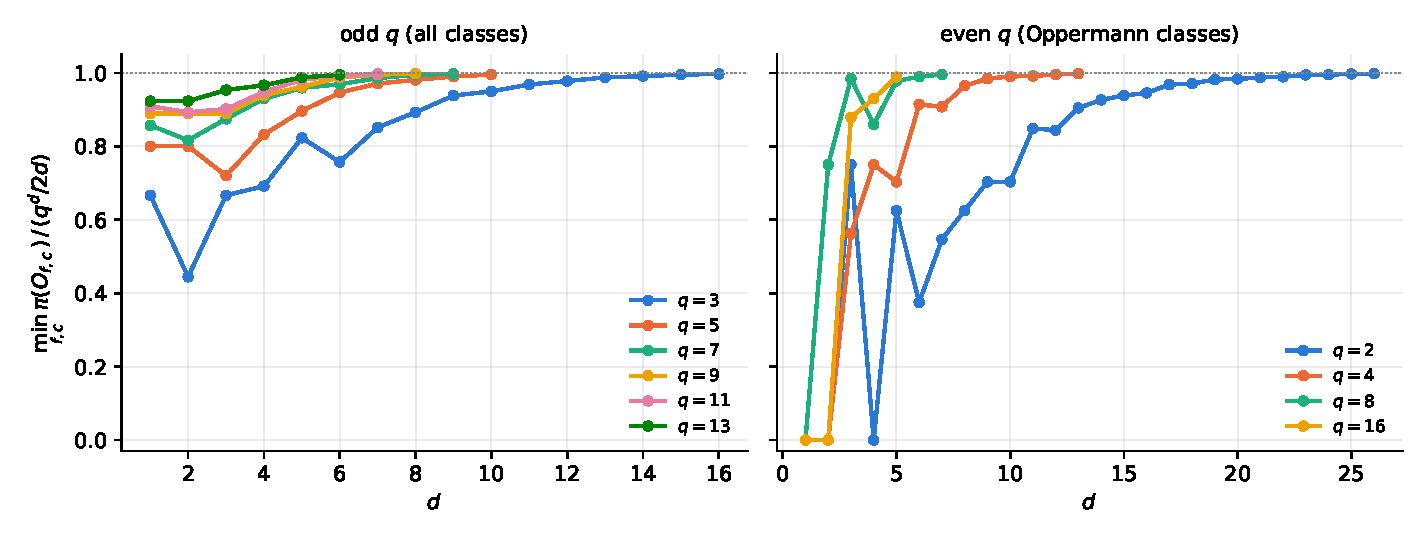
\includegraphics[width=\textwidth]{oppermann_min_ratio.pdf}
\caption{Normalised minimum $\min_{f,c}\pi(O_{f,c})/(q^d/2d)$ against $d$. Left: odd $q$. Right: even $q$; the
points at $0$ are the empty sub-intervals of Theorem~\ref{thm:main2}.}\label{fig:ratio}
\end{figure}

\begin{proof}[Proof of Theorems~\ref{thm:odd} and~\ref{thm:even}]
Exact computation as described above; the minima are in Tables~\ref{tab:odd} and~\ref{tab:even}, and the empty
classes in characteristic $2$ occur exactly at
\[
(q,d)\in\{(2,1),(2,2),(2,4),(4,1),(4,2),(8,1),(16,1),(16,2)\},
\]
one class each, which are the classes of Theorem~\ref{thm:main2}.
\end{proof}

The normalised minimum $\min_x\pi(x)/(q^d/2d)$ tends to $1$ in every column: the worst Oppermann sub-interval is
only slightly below average, far from the Weil bound discussed next.

\section{The square-root barrier}\label{sec:barrier}

In \eqref{eq:explicit} with $n=2d$, $l=d$, the main term is $q^d$. By Weil, every inverse zero $\gamma$ of $L(u,\chi)$,
$\chi\ne1$, has $|\gamma|\in\{1,\sqrt q\}$, so $|\psi_{2d}(\chi)|\le(d-1)q^d$, and averaging the $q^d-1$ nontrivial
characters gives only
\[
|\Psi(x)-q^d|\le(d-1)q^d .
\]
For $d\ge2$ the error term is at least the main term, for every $q$. This is the exact analogue of the situation
over $\Z$, where Oppermann's intervals have length $\sqrt x$ and the Riemann hypothesis falls short by
$\log x$. So no degree threshold beyond which $O_{f,c}\ne\emptyset$ follows from Weil's theorem, and
Theorem~\ref{thm:main2} shows that in characteristic $2$ no such threshold can be uniform in $q$ for $d=2$.

Results on the variance of $\Psi$ over Legendre intervals (an average over $f$) bound the number of intervals that
deviate by a given amount; they do not exclude a single empty interval.

For fixed degree and $q\to\infty$, Bank, Bary-Soroker and Rosenzweig \cite{BBR} prove the following. For monic
$f\in\F_q[t]$ of degree $k$ and $1\le m<k$, the number $N$ of irreducibles in $\{f+h:\deg h\le m\}$ satisfies
\[
\bigl|N-q^{m+1}/k\bigr|\le c(k)\,q^{m+1/2},
\]
provided that $m\ge2$ if $\gcd(q,k(k-1))>1$, and $m\ge3$ if $q$ is even and $\deg f'\le1$. They also note that the
estimate fails outside this range.

Our blocks $B_e=\{t^4+et^2+h:\deg h\le1\}$ have $k=4$ and $m=1$, and in characteristic $2$ the centre
$f=t^4+et^2$ has $f'=0$, so both conditions exclude them. Theorem~\ref{thm:main2}(B) gives the exact count at this
excluded point and shows how the asymptotic fails:
\begin{itemize}
\item for $q=4^j$ the block $e=0$ contains no irreducible, while the expected count is $q^2/4$;
\item for $q=2^{2j+1}$ the block $e=0$ contains $q(q-1)/2$, about twice the expected count.
\end{itemize}
The blocks $e\ne0$, with $q^2/4$ and $q(q-2)/4$ irreducibles, do agree with the asymptotic. The obstruction comes
from the additive structure of $t^4+et^2+\alpha t$ (Proposition~\ref{prop:agl}). For $m=1$, $k=4$ and $q$ even,
the conditions of \cite{BBR} therefore cannot be dropped.

Theorem~\ref{thm:main2}(C) has $q=2$ fixed, so it lies outside the $q\to\infty$ regime altogether.

\section{Questions}
\begin{enumerate}
\item In characteristic $2$, are (A)--(C) the only empty Oppermann sub-intervals for all $q$ and $d$? For $d=3$,
Lemma~\ref{lem:even} leaves $q^2$ classes; for $d=4$, $q^2$ classes, among them the zero block $Z_4$, which is
nonempty for $q=4,8,16$.
\item In odd characteristic, is every Oppermann sub-interval nonempty for all $q$ and $d$? Lemma~\ref{lem:odd}
turns this into a statement about all short intervals of length $q^{n/2}$.
\item Outside the characteristic-$2$ cases above, is there a constant $c>0$ with
$\min_x\pi(x)\ge c\,q^d/2d$ for all large $d$?
\end{enumerate}

\section*{Data and code}
\begin{itemize}
\item \texttt{hayes\_oppermann.py}: Theorems~\ref{thm:odd} and~\ref{thm:even}.
\item \texttt{verify\_pointwise\_oppermann.py}: brute-force census, $q^{2d}\le2^{26}$.
\item \texttt{compare\_bruteforce.py}: class-by-class cross-check.
\item \texttt{make\_tables.py}, \texttt{make\_figure.py}: Tables~\ref{tab:odd}, \ref{tab:even} and
Figure~\ref{fig:ratio}.
\item \texttt{char2\_d2\_blocks.py}, \texttt{char2\_d2\_theorem.py}: Theorem~\ref{thm:main2}(B).
\item \texttt{swan\_parity.py}: Theorem~\ref{thm:main2}(C) and Table~\ref{tab:zero}.
\item \texttt{hayes\_fft\_fq.py}, \texttt{fqlib.py}, \texttt{small\_q\_gf.py}: taken unchanged from \cite{ChenI}.
\end{itemize}
All scripts are in \texttt{code/}; their outputs are in \texttt{data/}.
\begin{thebibliography}{99}
\bibitem{BBR} E.~Bank, L.~Bary-Soroker, L.~Rosenzweig, \emph{Prime polynomials in short intervals and in arithmetic
progressions}, Duke Math. J. \textbf{164} (2015), 277--295.
\bibitem{Berlekamp76} E.~R. Berlekamp, \emph{An analog to the discriminant over fields of characteristic two},
J. Algebra \textbf{38} (1976), 315--317.
\bibitem{ChenI} R.~Chen, \emph{Primes in Legendre intervals over $\F_q[t]$: an exact explicit-formula algorithm,
verification for $d\le10$, and an anomaly in characteristic~2}, preprint (2026), DOI 10.5281/zenodo.23225896.
\bibitem{Hayes} D.~R. Hayes, \emph{The distribution of irreducibles in $GF[q,x]$}, Trans. Amer. Math. Soc.
\textbf{117} (1965), 101--127.
\bibitem{KR} J.~P. Keating, Z.~Rudnick, \emph{The variance of the number of prime polynomials in short intervals and
in residue classes}, Int. Math. Res. Not. IMRN \textbf{2014}, no.~1, 259--288.
\bibitem{Oppermann} L.~Oppermann, \emph{Om vor Kundskab om Primtallenes M\ae ngde mellem givne Gr\ae ndser},
Oversigt over det Kongelige Danske Videnskabernes Selskabs Forhandlinger (1882), 169--179.
\bibitem{Stickelberger} L.~Stickelberger, \emph{\"Uber eine neue Eigenschaft der Diskriminanten algebraischer
Zahlk\"orper}, Verhandlungen des ersten Internationalen Mathematiker-Kongresses, Z\"urich, 1897, 182--193.
\bibitem{Swan} R.~G. Swan, \emph{Factorization of polynomials over finite fields}, Pacific J. Math. \textbf{12}
(1962), 1099--1106.
\end{thebibliography}

\end{document}
